\chapter{\textbf{Etude des systèmes ANPR}}
    \section{Introduction}
    Encore appelé \acrfull{lapi} ou encore \acrfull{alpr}, l’ANPR est une technologie qui permet d’identifier les plaques d’immatriculation des véhicules en utilisant les techniques de traitement d’images et de vision par ordinateur. Inventés en 1976 au Royaume Uni au sein de la Police Scientific Development Branch \cite{wikianpr}, les systèmes ANPR ont fait leur chemin dans plusieurs autres pays dans le monde devenant ainsi un outil puissant et indispensable pour la sécurité du trafic routier. Nous allons à cet effet dédié ce chapitre pour répondre à quatre questions importantes autour de ces systèmes à savoir:
        \begin{enumerate}
            \item \textit{Quelle est l’architecture d’un système ANPR et de quoi se constitue-il principalement ?}
            \item \textit{Quels sont les systèmes ANPR existants déjà sur le marché ?}
            \item \textit{Dans quels champs de notre société un tel système serait-il utile ?}
            \item \textit{Quels sont les problèmes qui peuvent entacher le bon fonctionnement de ces systèmes}
        \end{enumerate}

    \section{Architecture et Composants}
Pour lire automatiquement les numéros des plaques d’immatriculation, un système ANPR s’étend généralement sur 4 grandes phases:
\begin{enumerate}
    \item \textbf{Acquisition de l’image}: C’est l’entrée de tout système ANPR. A travers une caméra, le système reçoit une séquence d’images.
    \item \textbf{Pré-traitement}: C’est une phase qui est déterminante pour la précision du système. Elle permet d’améliorer la qualité de l’image acquise pour faciliter les prochains traitements.
    \item \textbf{Détection de la plaque}: C’est l’étape la plus importante et en même la plus difficile d’un système ANPR. Elle consiste à identifier sur l’ensemble de l’image la position exacte de la plaque et par la suite l’isoler du reste de l’image. Dans la littérature, plusieurs méthodes ont été proposées pour réussir cette phase à savoir:
        \begin{itemize}
            \item[•] \textbf{La méthode d’extraction des régions d’intérêt}: La région d'intérêt dans une image donnée est la plaque d'immatriculation. Cette région se trouve par
            application d'un concept pour une image donnée, la région contenant une plaque d'immatriculation devra
            nombre maximum de bords par rapport à toute autre partie dans une image. L’application de ce concept à
            tous les segments extraits, les coordonnées de la région requise sont extraites. Ces valeurs de coordonnées
            sont ensuite utilisées pour extraire la plaque d'immatriculation.
            \item[•] \textbf{La méthode basée sur la texture}: La texture est une caractéristique qui peut être utilisée pour détecter les plaques d’immatriculation vue
            que les caractères d’une plaque ont une texture similaires. Dans cet algorithme, on traite les caractères
            d’une plaque comme une texture distincte du reste des objets contenus dans une image. La méthode est
            décomposée en quatre étapes qui sont les suivantes :
                \begin{itemize}
                    \item \textbf{Analyse de la texture de l’image};
                    \item \textbf{Décomposition de l’image en multi-segment};
                    \item \textbf{Choix du masque};
                    \item \textbf{Analyse des composantes connexes}.
                \end{itemize}
            \item[•] \textbf{La méthode basée sur le contour et le gradient}: Les conditions de luminance non uniforme et la distance variable entre la caméra et le véhicule peuvent
            influencer sur le résultat de la détection des plaques d’immatriculation. Pour cela, il existe une méthode
            de détection des plaques d’immatriculation basée sur les caractéristiques du contour et des propriétés des
            caractères. L’algorithme proposé est basé sur les caractéristiques suivantes :
                \begin{itemize}
                    \item Les pixels présentant les caractères de la plaque ont souvent une valeur de contraste plus élevée par rapport aux pixels voisins.
                    \item Le contour des caractères d’une plaque est toujours un contour fermé.
                    \item Il y’ a une relation de voisinage entre les caractères.
                \end{itemize}
            De plus, cette approche qui se base sur le contour et le gradient est composée de cinq processus qui sont :
                \begin{itemize}
                    \item \textbf{Détection de contour};
                    \item \textbf{Sélection des régions candidates de caractères de la plaque d’immatriculation};
                    \item \textbf{Calcul du gradient magnitude des composantes connexes};
                    \item \textbf{Extraction des caractères};
                    \item \textbf{Localisation de la plaque d’immatriculation de véhicules}.\cite{akacemMaster}
                \end{itemize}
            \item[•] \textbf{La méthode basée sur l’apprentissage profond}: Les méthodes précédentes sont dites déterministes car sont implémentées avec des fonctions mathématiques avec des paramètres fixés. A cet effet, dans l'article \cite{doi:10.1177/0361198120954202}, \Citeauthor{doi:10.1177/0361198120954202} proposent une méthode basée sur un modèle de Deep Learning pour la détection des plaques. En effet, à partir une masse de données d’images contenant les plaques d’immatriculation, on réalise un modèle à l’aide des algorithmes de détection des objets (Object Detection). Ce modèle servira par la suite pour détecter les plaques sur de nouvelles images. Cette approche est de plus en plus adoptée car plus efficace par rapport aux approches classiques déterministes.
        \end{itemize}
    \item \textbf{Reconnaissance des caractères}: Encore appelé \acrshort{ocr}, le but de cette phase est d’extraire sous format textuel (alphanumérique), le numéro de la plaque de d’immatriculation.Si certaines méthodes \cite{krimMaster, 10.1155/2018/6737314} utilisent l'approche classique qui passent par 3 phases (prétraitement, segmentation de caractères et reconnaissance de caractères), d’autres \cite{Alahyane2021OpenDF, doi:10.1177/0361198120954202} par contre optent pour une approche nouvelle en utilisant directement un modèle de réseaux de neurones pour la reconnaissance des caractères sur l'image de la plaque. Toutefois quelque soit la méthode, une étape de post-traitement sur le texte détecté est nécessaire pour faire d'éventuelles corrections sous la base de la norme d’immatriculation des véhicules spécifique au pays. A la fin de la chaîne, le texte obtenu et nettoyé est soit enregistré dans une base de données ou envoyé à un autre système pour un traitement ultérieur.

\end{enumerate}

\begin{figure}[H]
    \centering
    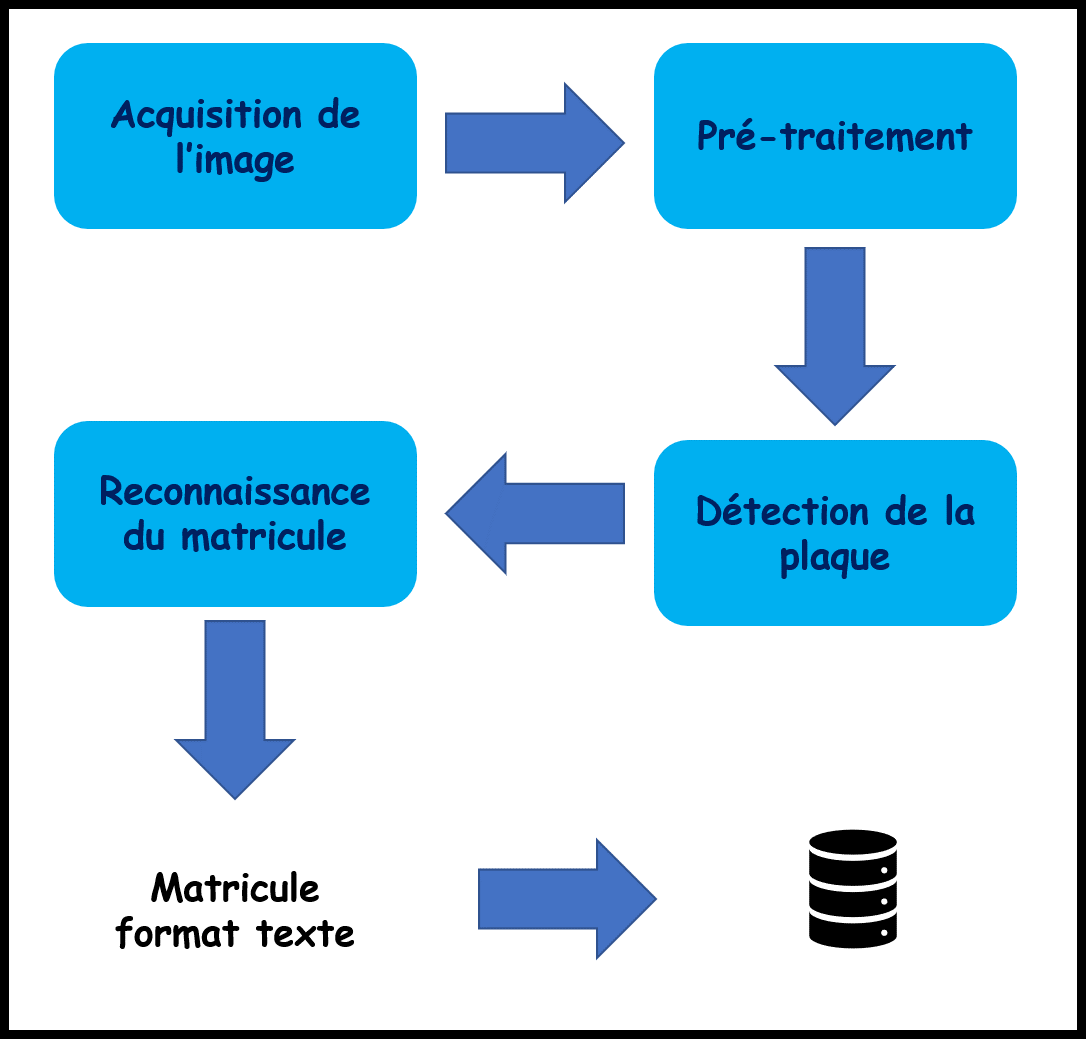
\includegraphics[scale=0.5]{architectureANPR}
    \caption{Architecture de fonctionnement d'un système ANPR}
\end{figure}
Tout système ANPR est constitué essentiellement de deux parties:
    \begin{enumerate}
        \item \textbf{Une partie matérielle}: Elle est composée d’une caméra qui permet d’acquérir les images et d’un ordinateur standard sur lequel s'exécute la partie logicielle du système.
        \item \textbf{Une partie logicielle}: C’est le programme qui traite les images en vue d’extraire les numéros des plaques d’immatriculation. Elle est la plupart du temps liée à une base de données où sont stockées les matricules.
    \end{enumerate}
    \input{chapters/02-EtudeANPR/02-SystèmesExistants}
    \section{Domaines d'application et Difficultés}
Depuis leur invention, les systèmes de reconnaissance automatique de plaques d’immatriculation n’ont cessé d’étendre leurs champs d’action. Ils sont même devenus incontournables dans les systèmes modernes et intelligents de gestion de trafic routier. Parmi les larges gammes d’applications de l’ANPR, on peut citer: 
    \begin{itemize}
        \item[•]\textbf{Vol de voitures}: le système est déployé sur le bord des routes, et réalise une comparaison en temps réel entre les voitures qui passent et la liste des voitures volées. Lorsqu’une correspondance est trouvée, une alerte est déclenchée pour informer l’agent de police de la voiture détectée et les raisons pour arrêter la voiture.
        \item[•]\textbf{Parking} : le numéro de la plaque d’immatriculation est utilisé pour le payement du stationnement au parking pour les gens ayant des cartes près-payée pour les parkings, afin de calculer les frais de stationnement en comparant les temps d’entrée et de sortie au parking.
        \item[•]\textbf{Péage} : le numéro de la voiture est utilisé pour calculer les frais de voyage dans une route à péage, ou utilisé pour revérifier le billet.
        \item[•]\textbf{Contrôle d’accès} : l’ouverture automatique d’une porte pour les membres agrées dans une zone de sécurité. Ce genre de système est mis en place pour aider les agents de sécurité. Les événements sont enregistrés sur une base de données et peuvent être utilisés pour rechercher l’historique des événements en cas de besoin.
        \item[•]\textbf{Contrôle des frontières} : le numéro de la voiture est enregistré à l’entrée ou à la sortie du pays, et utilisé pour surveiller les passages frontaliers. Chaque véhicule est enregistré dans une base de données centrale et lié à des informations supplémentaires telle que les données relatives aux passeports. Il est utilisé pour suivre tous les passages frontaliers.
        \item[•]\textbf{Code pénal de la route} : le numéro de plaque est utilisé pour produire une amende de violation de vitesse ou de feux rouges. Le processus manuel de préparation d’une amende de violation
        est remplacé par un processus automatisé qui réduit les surcharges et les délais. Les amendes peuvent être consultées et payées en ligne. \cite{HindeThesis}         
    \end{itemize} \par
Depuis certaines années, les pays dans le monde normalisent le format de leurs plaques d’immatriculation. Cette normalisation intervient d’une part sur l’uniformisation des couleurs possibles et d’autre part la liste et le nombre de caractères que l’on peut trouver sur une plaque valide. Cette régularisation des plaques minéralogiques a rendu les systèmes ANPR plus spécifiques et donc plus performants. Néanmoins, comme tout système faisant du traitement d’image, les systèmes ANPR font face à des difficultés comme:
    \begin{itemize}
        \item[•] \textbf{Une mauvaise résolution de l’image} qui est la conséquence soit d’une caméra de mauvaise qualité soit de l’éloignement de la plaque par rapport à la caméra;
        \item[•] \textbf{Des images floues} principalement causées par le mouvement;
        \item[•] \textbf{Les mauvaises conditions climatiques}: Les phénomènes naturels comme la pluie, la poussière et le brouillard peuvent empêcher une bonne capture des images et donc impacter négativement la précision d'un système ANPR.
        \item[•] \textbf{La différence de polices de caractères de la plaque} à cause de la fantaisie faite par certains usagers. \cite{wikianpr}   
    \end{itemize}
Si certains de ces problèmes peuvent être surmontés en agissant sur la partie logiciel du système, d’autres par contre nécessitent une intervention au niveau matériel. 
    \section{Difficultés}
Depuis certaines années, les pays dans le monde normalisent le format de leurs plaques d’immatriculation. Cette normalisation intervient d’une part sur l’uniformisation des couleurs possibles et d’autre part la liste et le nombre de caractères que l’on peut trouver sur une plaque valide. Cette régularisation des plaques minéralogiques a rendu les systèmes ANPR plus spécifiques et donc plus performants. Néanmoins, comme tout système faisant du traitement d’image, les systèmes ANPR font face à des difficultés comme:
    \begin{itemize}
        \item[•] \textbf{Une mauvaise résolution de l’image} qui est la conséquence soit d’une caméra de mauvaise qualité soit de l’éloignement de la plaque par rapport à la caméra;
        \item[•] \textbf{Des images floues} principalement causées par le mouvement;
        \item[•] \textbf{Un mauvais éclairage et un faible contraste } à cause d'une surexposition, d'un reflet, ou d'ombres;
        Les objets qui cachent une partie de la plaque
        \item[•] \textbf{La différence de polices de caractères de la plaque} à cause de la fantaisie faite par certains usagers. \cite{wikianpr}   
    \end{itemize}
Si certains de ces problèmes peuvent être surmontés en agissant sur la partie logiciel du système, d’autres par contre nécessitent une intervention au niveau matériel. 



    \section{Conclusion}
    Ce chapitre nous a permis de comprendre que les systèmes ANPR ne sont pas une nouveauté. En réalité, plusieurs études ont déjà été menées de long en large. Ces travaux ont ainsi contribué d’une part à standardiser plus au moins l’architecture générale d’un système ANPR et d’autre part à déterminer les composants essentiels de ce système. Ces travaux sont aussi le socle sur lequel plusieurs entreprises ont construit leur propre solution ANPR qui fait face plus ou moins bien aux difficultés que rencontrent la majorité des technologies de traitement d’images. Le prochain chapitre sera donc une occasion d'exposer les différentes techniques de traitements d'images.